% !TEX encoding = UTF-8 Unicode
\level{1}{Preventivo}
	\level{2}{Dettaglio fasi}
		\level{3}{Fase C}
			\level{4}{Suddivisione lavoro}
				Nella \insphase{Fase C} ogni componente del gruppo \groupname{} coprirà i seguenti ruoli:
				\begin{table}[H]
					\begin{center}
						\begin{tabular}{| l | c | c | c | c | c | c | c |}
							\hline
							Componente 				& PM	& Am	 & An 	& Pt 		& Pm 	& Ve 	& Ore Totali componente \\ \hline
							
							Bigarella Chiara 			& 0		& 0		& 10 		& 17 		& 0		& 6 		& 33 \\
							Bucco Riccardo 			& 15 		& 0		& 0		& 15 		& 0		& 5 		& 35 \\
							Carlon Chiara	 			& 0		& 7 		& 12 		& 0		& 0		& 9 		& 28 \\
							Dal Bianco Davide 			& 0		& 0		& 0		& 20 		& 0		& 5		& 25 \\
							Moretto Alessandro 			& 0		& 3 		& 10 		& 12 		& 0		& 5 		& 30 \\
							Pavanello Fabio Matteo	 	& 0		& 0		& 25 		& 0		& 0		& 0		& 25 \\
							Rubin Marco				& 9 		& 0		& 12 		& 0		& 0		& 7 		& 28 \\ \hline \hline
							
							Ore Totali Ruolo 			& 24 		& 10 		& 69 		& 64 		& 0		& 37		& 204\\ \hline
						\end{tabular}
					\end{center}
					\caption{Suddivisione ore di lavoro Fase C}
				\end{table}
				Riassumendo con un Bar Chart:
				\begin{figure}[H]\centering
					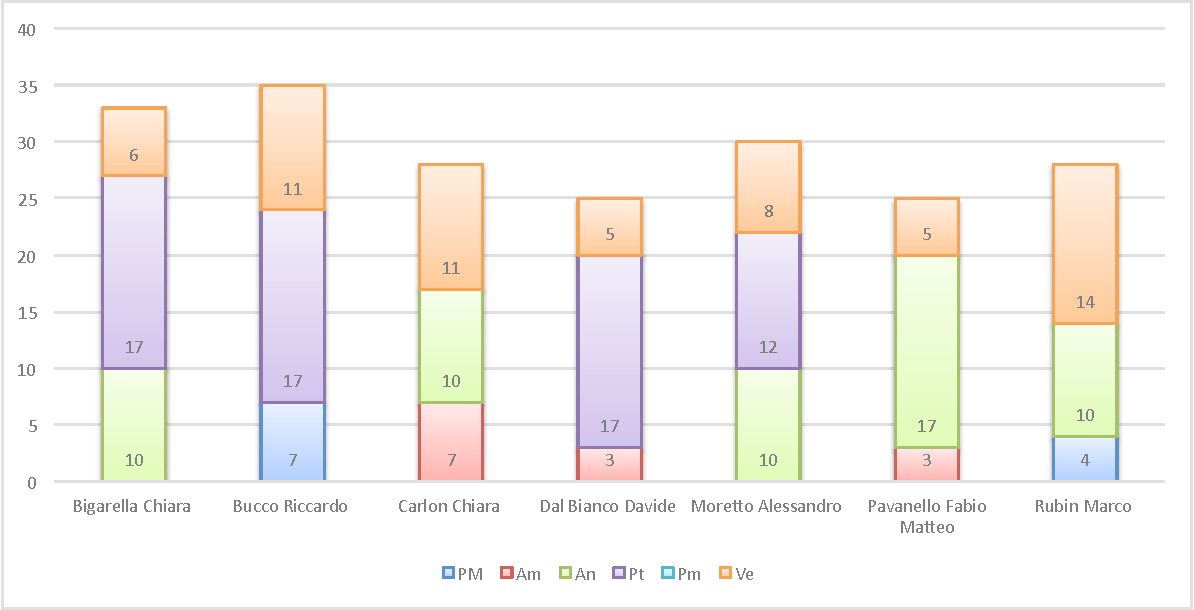
\includegraphics[width=\textwidth]{PianoDiProgetto/Pics/ChartOreFaseC.pdf}
					\caption{Bar Chart ore persona Fase C}
				\end{figure}
			\level{4}{Prospetto economico}
				Nella \insphase{Fase C} il costo di ogni ruolo è il seguente:
				\begin{table}[H]
					\begin{center}
						\begin{tabular}{| l | c | c |}
							\hline
							Ruolo 			& Ore 	& Costi  \\ \hline
							
							Project Manager	& 24 		& \euro{} 720,00 	\\
							Amministratore 		& 10 		& \euro{} 200,00 	\\
							Analista	 		& 69 		& \euro{} 1~725,00 	\\
							Progettista 		& 64 		& \euro{} 1~408,00  	\\
							Programmatore		& 0		& \euro{} 0,00	\\
							Verificatore		& 37 		& \euro{} 555,00 	\\ \hline \hline
							
							Totale	 		& 204 	& \euro{} 4~608,00 	\\ \hline
						\end{tabular}
					\end{center}
					\caption{Costi per ruolo Fase C}
				\end{table}
				Riassumendo le ore per ruolo con un Pie Chart:
				\begin{figure}[H]\centering
					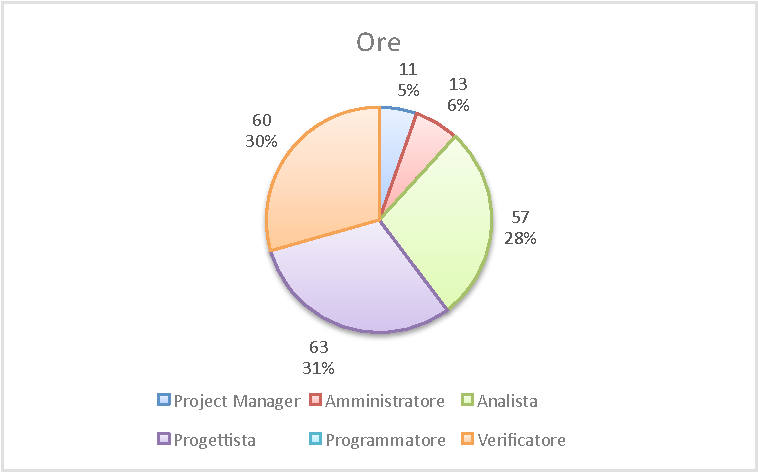
\includegraphics[width=\textwidth]{PianoDiProgetto/Pics/ChartTotOreFaseC.pdf}
					\caption{Pie Chart ore per ruolo Fase C}
				\end{figure}
				Riassumendo i costi per ruolo con un Pie Chart:
				\begin{figure}[H]\centering
					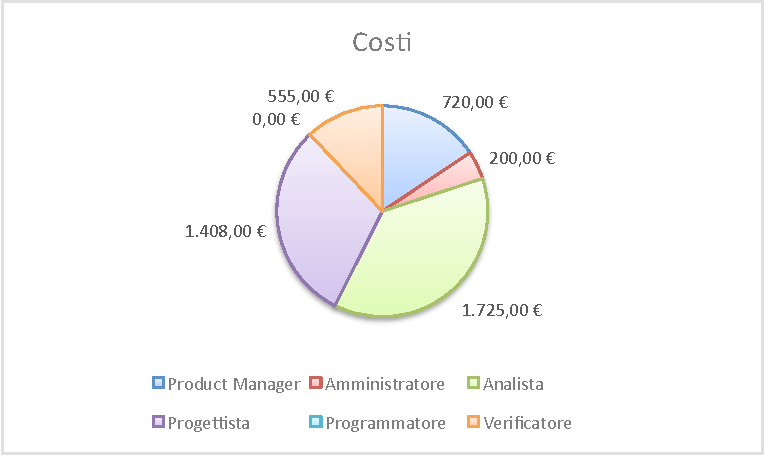
\includegraphics[width=\textwidth]{PianoDiProgetto/Pics/ChartTotCostiFaseC.pdf}
					\caption{Pie Chart costi per ruolo Fase C}
				\end{figure}
		\level{3}{Fase D}
			\level{4}{Suddivisione lavoro}
				Nella \insphase{Fase D} ogni componente del gruppo \groupname{} coprirà i seguenti ruoli:
				\begin{table}[H]
					\begin{center}
						\begin{tabular}{| l | c | c | c | c | c | c | c |}
							\hline
							Componente 				& PM	& Am 	& An 	& Pt 		& Pm 	& Ve 	& Ore Totali componente \\ \hline
							
							Bigarella Chiara 			& 0		& 0		& 0		& 9 		& 14 		& 8 		& 31 \\
							Bucco Riccardo 			& 0		& 0		& 0		& 7 		& 12		& 15 		& 34 \\
							Carlon Chiara	 			& 0		& 0		& 13 		& 0		& 11 		& 6 		& 30 \\
							Dal Bianco Davide 			& 17 		& 0		& 0		& 13 		& 0		& 3 		& 33 \\
							Moretto Alessandro 			& 0		& 5 		& 0		& 17 		& 4 		& 8 		& 34 \\
							Pavanello Fabio Matteo	 	& 0		& 0		& 12 		& 0		& 8 		& 13 		& 33 \\
							Rubin Marco				& 0		& 4 		& 0		& 17 		& 0		& 8 		& 29 \\ \hline \hline
							
							Ore Totali Ruolo 			& 17 		& 9 		& 25 		& 63 		& 49 		& 61 		& 224	\\ \hline
						\end{tabular}
					\end{center}
					\caption{Suddivisione ore di lavoro Fase D}
				\end{table}
				Riassumendo con un Bar Chart:
				\begin{figure}[H]\centering
					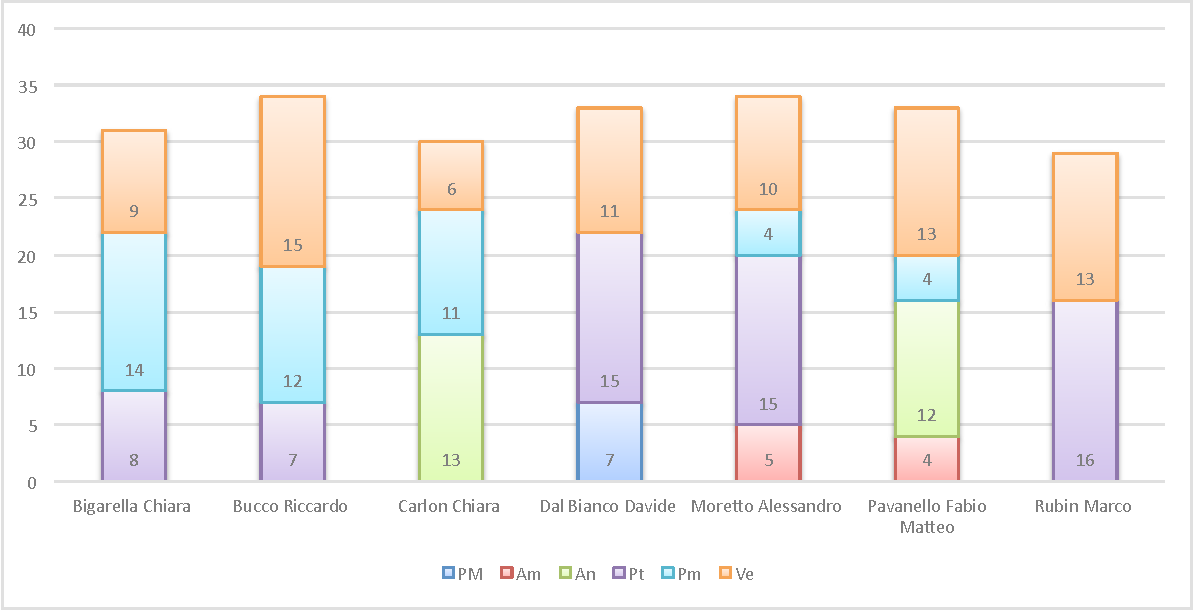
\includegraphics[width=\textwidth]{PianoDiProgetto/Pics/ChartOreFaseD.pdf}
					\caption{Bar Chart ore persona Fase D}
				\end{figure}
			\level{4}{Prospetto economico}
				Nella \insphase{Fase D} il costo di ogni ruolo è il seguente:
				\begin{table}[H]
					\begin{center}
						\begin{tabular}{| l | c | c |}
							\hline
							Ruolo 			& Ore 	& Costi  \\ \hline
							
							Project Manager	& 17 		& \euro{} 510,00 	\\
							Amministratore 		& 9 		& \euro{} 180,00 	\\
							Analista	 		& 25 		& \euro{} 625,00 	\\
							Progettista 		& 63 		& \euro{} 1~386,00  	\\
							Programmatore		& 49 		& \euro{} 735,00 	\\
							Verificatore		& 61 		& \euro{} 915,00 	\\ \hline \hline
							
							Totale	 		& 224 	& \euro{} 4~351,00 	\\ \hline
						\end{tabular}
					\end{center}
					\caption{Costi per ruolo Fase D}
				\end{table}
				Riassumendo le ore per ruolo con un Pie Chart:
				\begin{figure}[H]\centering
					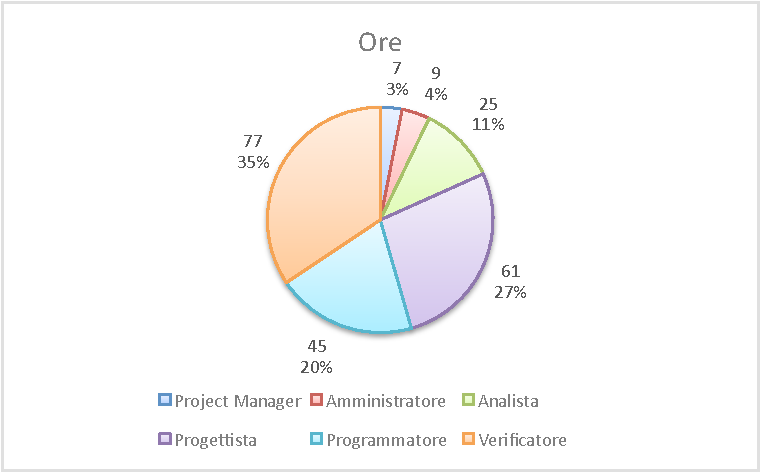
\includegraphics[width=\textwidth]{PianoDiProgetto/Pics/ChartTotOreFaseD.pdf}
					\caption{Pie Chart ore per ruolo Fase D}
				\end{figure}
				Riassumendo i costi per ruolo con un Pie Chart:
				\begin{figure}[H]\centering
					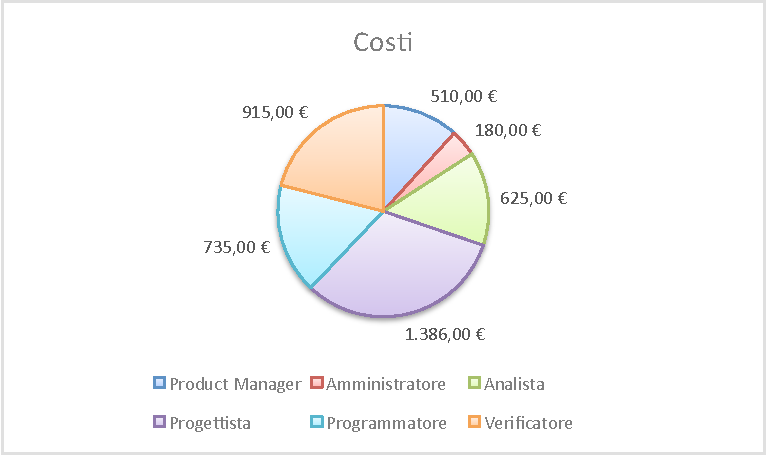
\includegraphics[width=\textwidth]{PianoDiProgetto/Pics/ChartTotCostiFaseD.pdf}
					\caption{Pie Chart costi per ruolo Fase D}
				\end{figure}
		\level{3}{Fase E}
			\level{4}{Suddivisione lavoro}
				Nella \insphase{Fase E} ogni componente del gruppo \groupname{} coprirà i seguenti ruoli:
				\begin{table}[H]
					\begin{center}
						\begin{tabular}{| l | c | c | c | c | c | c | c |}
							\hline
							Componente 				& PM	& Am	& An 	& Pt 		& Pm 	& Ve 	& Ore Totali componente \\ \hline
							
							Bigarella Chiara 			& 10 		& 0		& 0		& 0		& 3 		& 0		& 13 \\
							Bucco Riccardo 			& 0		& 0		& 0		& 0		& 2		& 12 		& 14 \\
							Carlon Chiara	 			& 0		& 2 		& 0		& 4 		& 2 		& 8 		& 16 \\
							Dal Bianco Davide 			& 0		& 0		& 0		& 0		& 5 		& 8 		& 13 \\
							Moretto Alessandro 			& 0		& 0		& 13 		& 0		& 0		& 0		& 13 \\
							Pavanello Fabio Matteo	 	& 0		& 0		& 0		& 0		& 3 		&11 		& 14 \\
							Rubin Marco				& 0		& 3 		& 0		& 6 		& 3 		& 6		& 18 \\ \hline \hline
							
							Ore Totali Ruolo 			& 10 		& 5 		& 13 		& 10 		& 18 		& 45 		& 101\\ \hline
						\end{tabular}
					\end{center}
					\caption{Suddivisione ore di lavoro Fase E}
				\end{table}
				Riassumendo con un Bar Chart:
				\begin{figure}[H]\centering
					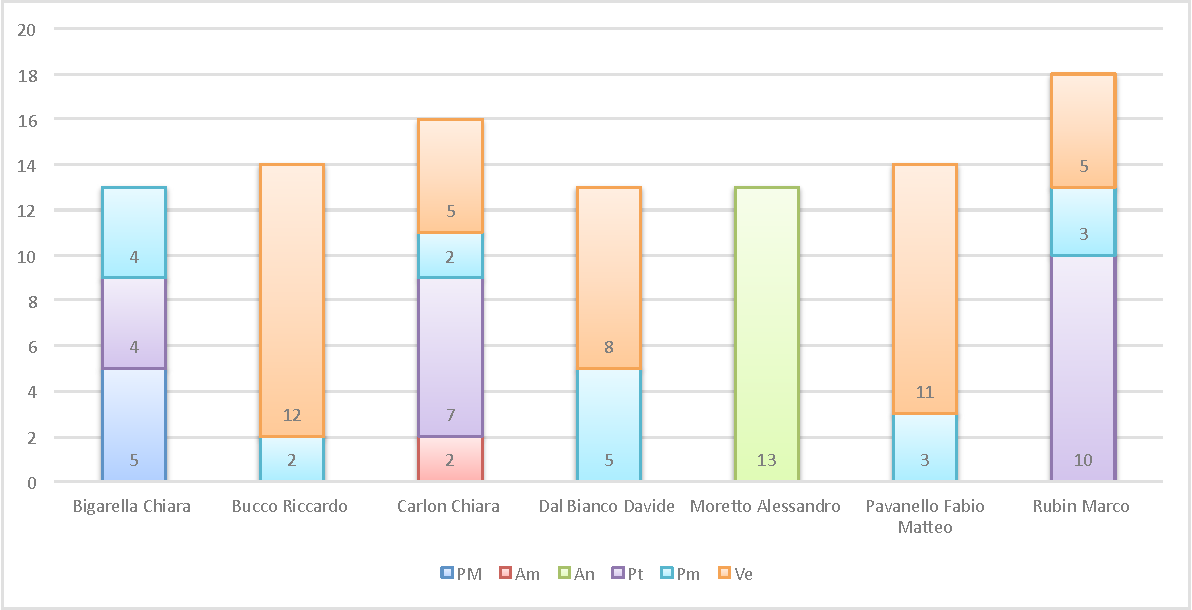
\includegraphics[width=\textwidth]{PianoDiProgetto/Pics/ChartOreFaseE.pdf}
					\caption{Bar Chart ore persona Fase E}
				\end{figure}
			\level{4}{Prospetto economico}
				Nella \insphase{Fase E} il costo di ogni ruolo è il seguente:
				\begin{table}[H]
					\begin{center}
						\begin{tabular}{| l | c | c |}
							\hline
							Ruolo 			& Ore 	& Costi  \\ \hline
							
							Project Manager	& 10 		& \euro{} 300,00 	\\
							Amministratore 		& 5 		& \euro{} 100,00 	\\
							Analista	 		& 13 		& \euro{} 325,00 	\\
							Progettista 		& 10 		& \euro{} 220,00  	\\
							Programmatore		& 18		& \euro{} 270,00 	\\
							Verificatore		& 45 		& \euro{} 675,00 	\\ \hline \hline
							
							Totale	 		& 101 	& \euro{} 1~890,00 	\\ \hline
						\end{tabular}
					\end{center}
					\caption{Costi per ruolo Fase E}
				\end{table}
				Riassumendo le ore per ruolo con un Pie Chart:
				\begin{figure}[H]\centering
					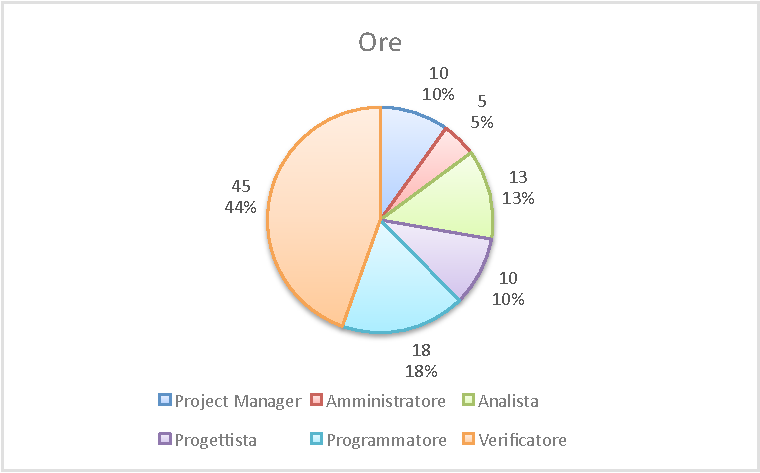
\includegraphics[width=\textwidth]{PianoDiProgetto/Pics/ChartTotOreFaseE.pdf}
					\caption{Pie Chart ore per ruolo Fase E}
				\end{figure}
				Riassumendo i costi per ruolo con un Pie Chart:
				\begin{figure}[H]\centering
					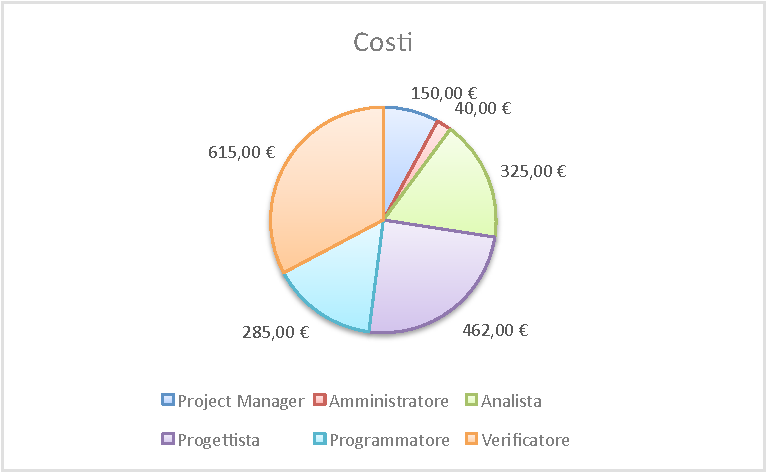
\includegraphics[width=\textwidth]{PianoDiProgetto/Pics/ChartTotCostiFaseE.pdf}
					\caption{Pie Chart costi per ruolo Fase E}
				\end{figure}
		\level{3}{Fase F}
			\level{4}{Suddivisione lavoro}
				Nella \insphase{Fase F} ogni componente del gruppo \groupname{} coprirà i seguenti ruoli:
				\begin{table}[H]
					\begin{center}
						\begin{tabular}{| l | c | c | c | c | c | c | c |}
							\hline
							Componente 				& PM	& Am 	& An 	& Pt 		& Pm 	& Ve 	& Ore Totali componente \\ \hline
							
							Bigarella Chiara 			& 0		& 0		& 0		& 6 		& 0		& 8 		& 14 \\
							Bucco Riccardo 			& 0		& 0		& 0		& 4 		& 0		& 7 		& 11 \\
							Carlon Chiara	 			& 0		& 5 		& 0		& 10 		& 0		& 3 		& 18 \\
							Dal Bianco Davide 			& 0		& 0		& 0		& 0		& 12 		& 9 		& 21 \\
							Moretto Alessandro 			& 0		& 0		& 0		& 0		& 11 		& 5		& 16 \\
							Pavanello Fabio Matteo	 	& 13 		& 0		& 0		& 0		& 5 		& 4 		& 22 \\
							Rubin Marco				& 0		& 0		& 13 		& 0		& 0		& 4 		& 17 \\ \hline \hline
							
							Ore Totali Ruolo 			& 13 		& 5 		& 13 		& 20 		& 28 		& 40 		& 119\\ \hline
						\end{tabular}
					\end{center}
					\caption{Suddivisione ore di lavoro Fase F}
				\end{table}
				Riassumendo con un Bar Chart:
				\begin{figure}[H]\centering
					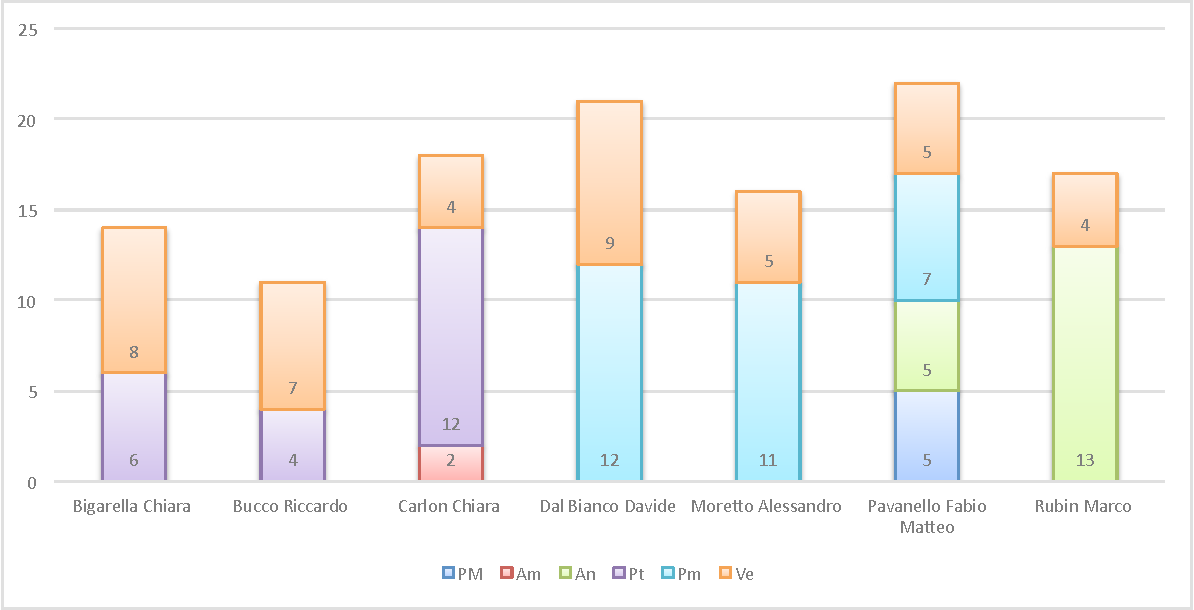
\includegraphics[width=\textwidth]{PianoDiProgetto/Pics/ChartOreFaseF.pdf}
					\caption{Bar Chart ore persona Fase F}
				\end{figure}
			\level{4}{Prospetto economico}
				Nella \insphase{Fase F} il costo di ogni ruolo è il seguente:
				\begin{table}[H]
					\begin{center}
						\begin{tabular}{| l | c | c |}
							\hline
							Ruolo 			& Ore 		& Costi  \\ \hline
							
							Project Manager	& 13 		& \euro{} 390,00 	\\
							Amministratore 		& 5 		& \euro{} 100,00 	\\
							Analista	 		& 13 		& \euro{} 325,00 	\\
							Progettista 		& 20 		& \euro{} 440,00  	\\
							Programmatore		& 28 		& \euro{} 420,00 	\\
							Verificatore		& 40 		& \euro{} 600,00 	\\ \hline \hline
							
							Totale	 		& 119 	& \euro{} 2~275,00 	\\ \hline
						\end{tabular}
					\end{center}
					\caption{Costi per ruolo Fase F}
				\end{table}
				Riassumendo le ore per ruolo con un Pie Chart:
				\begin{figure}[H]\centering
					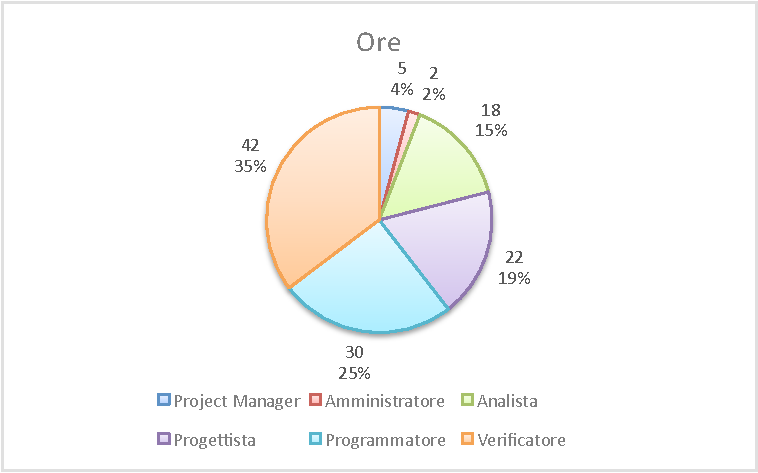
\includegraphics[width=\textwidth]{PianoDiProgetto/Pics/ChartTotOreFaseF.pdf}
					\caption{Pie Chart ore per ruolo Fase F}
				\end{figure}
				Riassumendo i costi per ruolo con un Pie Chart:
				\begin{figure}[H]\centering
					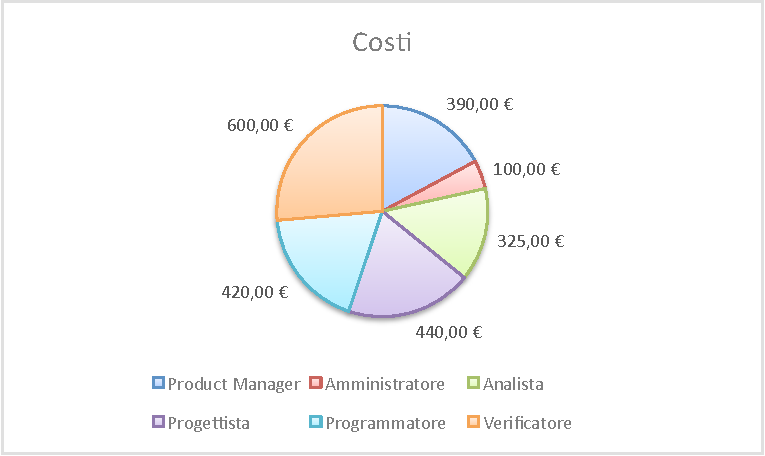
\includegraphics[width=\textwidth]{PianoDiProgetto/Pics/ChartTotCostiFaseF.pdf}
					\caption{Pie Chart costi per ruolo Fase F}
				\end{figure}
		\level{3}{Fase G}
			\level{4}{Suddivisione lavoro}
				Nella \insphase{Fase G} ogni componente del gruppo \groupname{} coprirà i seguenti ruoli:
				\begin{table}[H]
					\begin{center}
						\begin{tabular}{| l | c | c | c | c | c | c | c |}
							\hline
							Componente 				& PM	& Am 	& An 	& Pt 		& Pm 	& Ve 	& Ore Totali componente \\ \hline
							
							Bigarella Chiara 			& 0		& 0		& 0		& 0		& 5 		& 9 		& 14 \\
							Bucco Riccardo 			& 0		& 0		& 0		& 0		& 7		& 4 		& 11 \\
							Carlon Chiara	 			& 10 		& 0		& 0		& 0		& 0		& 3 		& 13 \\
							Dal Bianco Davide 			& 0		& 0		& 0		& 0		& 0		& 13 		& 13 \\
							Moretto Alessandro 			& 0		& 3 		& 0		& 0		& 0		& 9 		& 12 \\
							Pavanello Fabio Matteo	 	& 0		& 0		& 0		& 9 		& 0		& 2 		& 11 \\
							Rubin Marco				& 0		& 0		& 0		& 0		& 5 		& 8 		& 13 \\ \hline \hline
							
							Ore Totali Ruolo 			& 10 		& 3 		& 0		& 9 		& 17 		& 48 		& 87\\ \hline
						\end{tabular}
					\end{center}
					\caption{Suddivisione ore di lavoro Fase G}
				\end{table}
				Riassumendo con un Bar Chart:
				\begin{figure}[H]\centering
					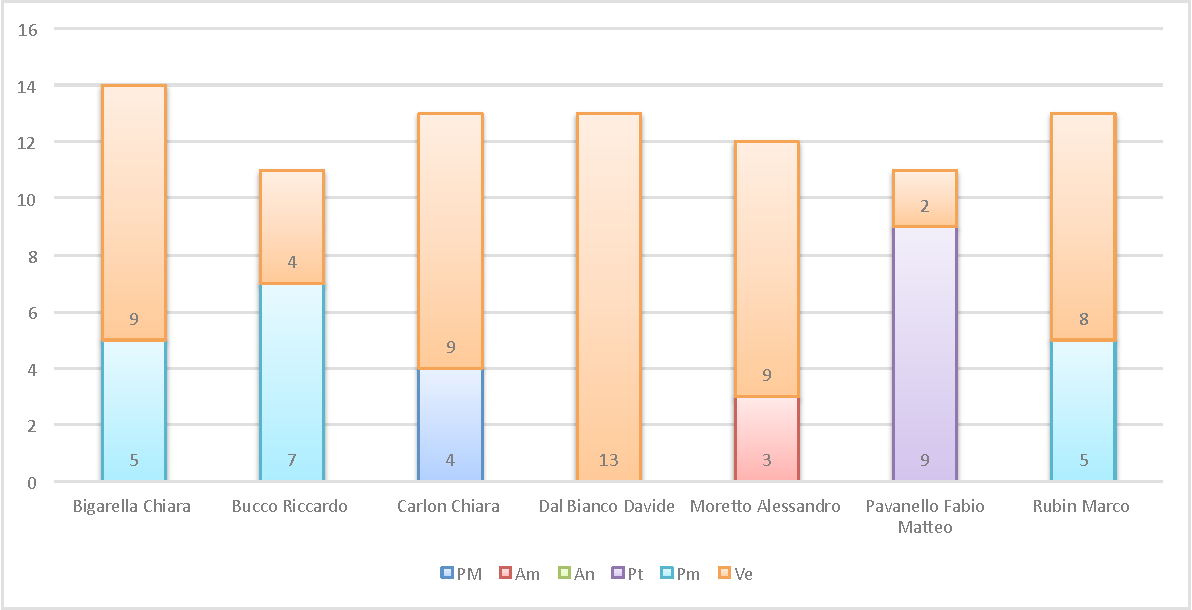
\includegraphics[width=\textwidth]{PianoDiProgetto/Pics/ChartOreFaseG.pdf}
					\caption{Bar Chart ore persona Fase G}
				\end{figure}
			\level{4}{Prospetto economico}
				Nella \insphase{Fase G} il costo di ogni ruolo è il seguente:
				\begin{table}[H]
					\begin{center}
						\begin{tabular}{| l | c | c |}
							\hline
							Ruolo 			& Ore 	& Costi  \\ \hline
							
							Project Manager	& 10 		& \euro{} 300,00 	\\
							Amministratore 		& 3 		& \euro{} 60,00 	\\
							Analista	 		& 0		& \euro{} 0,00	\\
							Progettista 		& 9 		& \euro{} 198,00  	\\
							Programmatore		& 17 		& \euro{} 225,00 	\\
							Verificatore		& 48 		& \euro{} 720,00 	\\ \hline \hline
							
							Totale	 		& 87 		& \euro{} 1~533,00 	\\ \hline
						\end{tabular}
					\end{center}
					\caption{Costi per ruolo Fase G}
				\end{table}
				Riassumendo le ore per ruolo con un Pie Chart:
				\begin{figure}[H]\centering
					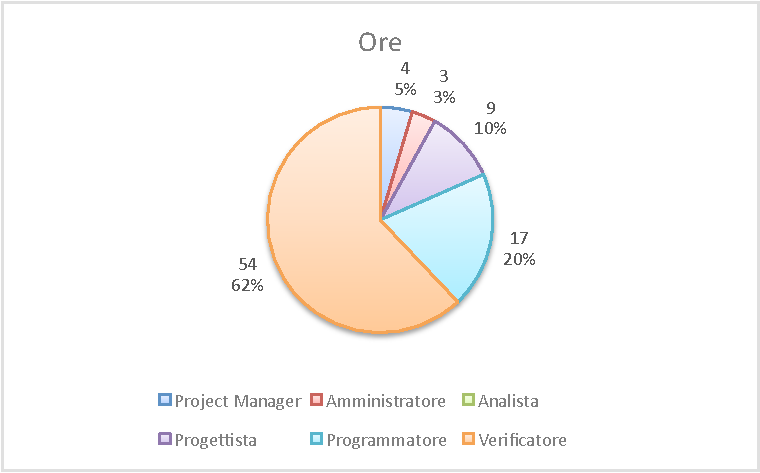
\includegraphics[width=\textwidth]{PianoDiProgetto/Pics/ChartTotOreFaseG.pdf}
					\caption{Pie Chart ore per ruolo Fase G}
				\end{figure}
				Riassumendo i costi per ruolo con un Pie Chart:
				\begin{figure}[H]\centering
					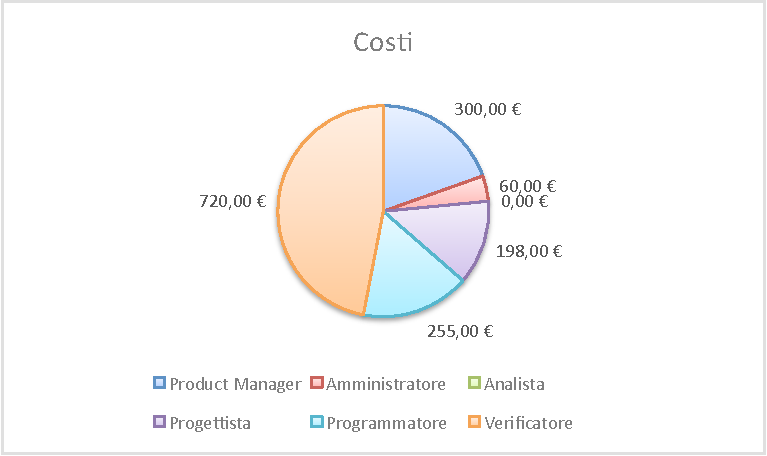
\includegraphics[width=\textwidth]{PianoDiProgetto/Pics/ChartTotCostiFaseG.pdf}
					\caption{Pie Chart costi per ruolo Fase G}
				\end{figure}
	\level{2}{Totale}
		\level{3}{Suddivisione lavoro}
			La suddivisione delle ore rendicontate per ruolo di ogni componente del gruppo \groupname{} saranno le seguenti:
			\begin{table}[H]
				\begin{center}
					\begin{tabular}{| l | c | c | c | c | c | c | c |}
						\hline
						Componente 				& PM	& Am 	& An 	& Pt 		& Pm 	& Ve 	& Ore Totali componente \\ \hline
						
						Bigarella Chiara 			& 10 		& 0		& 10 		& 32 		& 22 		& 31 		& 105 \\
						Bucco Riccardo 			& 15 		& 0		& 0		& 26 		& 21		& 43 		& 105 \\
						Carlon Chiara	 			& 10 		& 14 		& 25 		& 14 		& 13 		& 29 		& 105 \\
						Dal Bianco Davide 			& 17 		& 0		& 0		& 33 		& 17 		& 38 		& 105 \\
						Moretto Alessandro 			& 0		& 11 		& 23 		& 29 		& 15 		& 27 		& 105 \\
						Pavanello Fabio Matteo	 	& 13 		& 0		& 37 		& 9 		& 16 		& 30 		& 105 \\
						Rubin Marco				& 9 		& 7 		& 25 		& 23 		& 8 		& 33		& 105 \\ \hline \hline
						
						Ore Totali Ruolo 			& 74 		& 32 		& 120 	& 166 	& 112 	& 231 	& 735\\ \hline
					\end{tabular}
				\end{center}
				\caption{Suddivisione ore totali rendicontate}
			\end{table}
			Riassumendo con un Bar Chart:
			\begin{figure}[H]\centering
				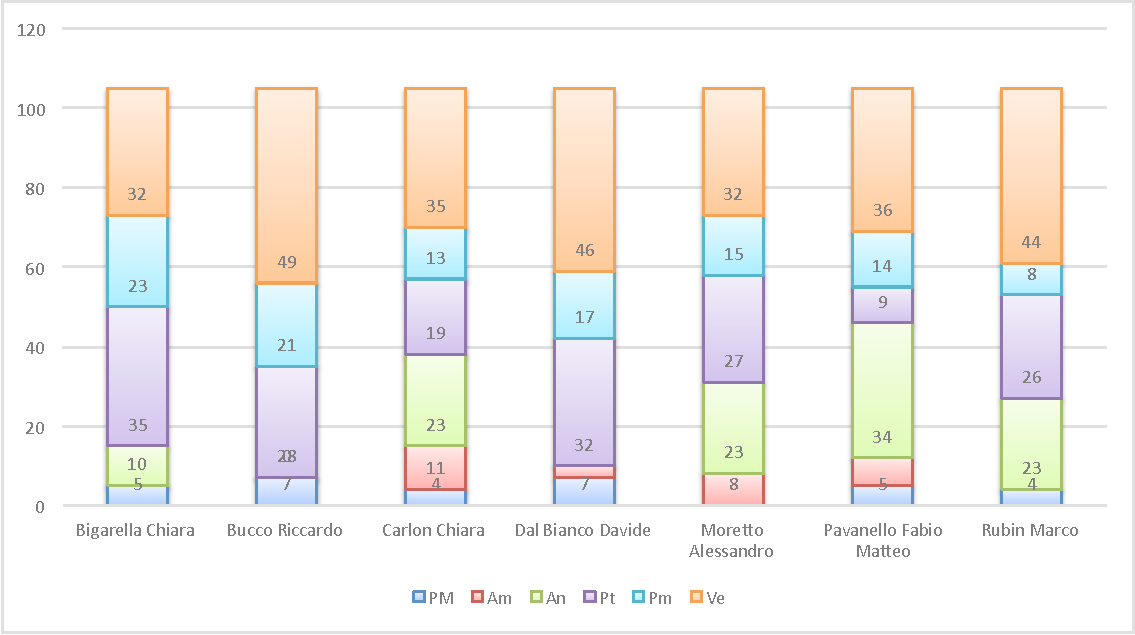
\includegraphics[width=\textwidth]{PianoDiProgetto/Pics/ChartOreRendic.pdf}
				\caption{Bar Chart ore totali rendicontate}
			\end{figure}
		\level{3}{Prospetto economico}
			Le ore rendicontate per ogni ruolo sono le seguenti:
			\begin{table}[H]
				\begin{center}
					\begin{tabular}{| l | c | c |}
						\hline
						Ruolo 			& Ore 		& Costi  \\ \hline
						
						Project Manager	& 74 			& \euro{} 2~220,00 	\\
						Amministratore 		& 32 			& \euro{} 640,00 	\\
						Analista	 		& 120 		& \euro{} 3~000,00 	\\
						Progettista 		& 166 		& \euro{} 3~652,00  	\\
						Programmatore		& 112 		& \euro{} 1~680,00 	\\
						Verificatore		& 231 		& \euro{} 3~465,00 	\\ \hline \hline
						
						Totale	 		& 735 		& \euro{} 14~657,00 	\\ \hline
					\end{tabular}
				\end{center}
				\caption{Spese rendicontate per ruolo}
			\end{table}
			Riassumendo le ore rendicontate per ruolo con un Pie Chart:
			\begin{figure}[H]\centering
				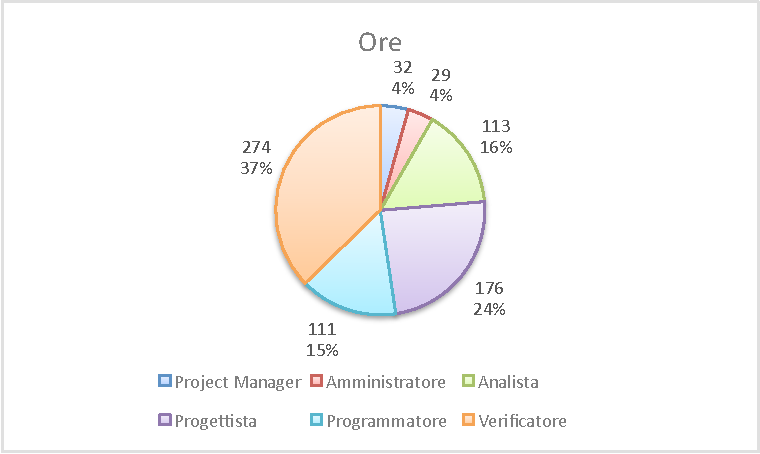
\includegraphics[width=\textwidth]{PianoDiProgetto/Pics/ChartTotOreRendic.pdf}
				\caption{Pie Chart ore rendicontate}
			\end{figure}
			Riassumendo i costi rendicontati per ruolo con un Pie Chart:
			\begin{figure}[H]\centering
				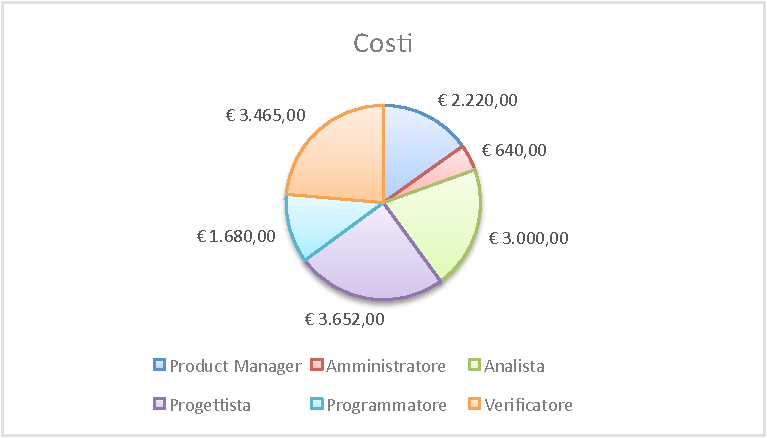
\includegraphics[width=\textwidth]{PianoDiProgetto/Pics/ChartTotCostiRendic.pdf}
				\caption{Pie Chart spese rendicontate per ruolo}
			\end{figure}
		\level{3}{Conclusione}
		Il costo totale del progetto è di \euro{} 14~657,00.